\chapter{ValDX Protocols and Supporting Analyses}
\label{app:valdx-protocols}

\section{Dataset Processing}
\label{app:valdx-hdx-data}

We applied filtering criteria so that the data used for ensemble optimisation were informative and compatible with the Best--Vendruscolo (BV) model.\supercite{bestStructuralInterpretationHydrogen2006} We performed all fractional uptake calculations and normalisations before any filtering.

As detailed in \cref{tab:valdx-data}, BRD4, HOIP, and LXR$\alpha$ uptake values were normalised using peptide-level fully deuterated controls and were therefore corrected for back-exchange. BPTI instead comprises NMR-derived residue-level protection factors, for which a FullD control is not applicable. The MBP data did not include a FullD control and were scaled to the maximum measured time point. This scaling does not correct back-exchange. Consequently, the absolute MBP uptake values may be systematically underestimated, with peptide-specific deuterium loss potentially distorting relative uptake as well as its overall scale. We retained MBP as a publicly available benchmark spanning a distinct protein system, but used it only during protocol development and do not report its results in \cref{ch:valdx}. Although $\text{Work}_\text{scale}$ (\cref{sec:valdx-work}) reports a global shift in predicted protection, it cannot correct peptide-specific back-exchange; uncorrected MBP results must therefore be interpreted with this limitation.

\begin{itemize}
    \item \textbf{Time point filtering.} We removed time points where the replicate precision (relative standard deviation, RSD) exceeded 5\%. This threshold typically corresponds to very short or very long deuteration times. Excluding poorly informative time points removes data that the single-exponential BV model describes poorly. This threshold aligns with high-precision HDX-MS estimates.\supercite{hudgensInterlaboratoryComparisonHydrogenDeuterium2019}
    \item \textbf{Peptide filtering.} We removed peptides that were short ($<5$ residues) or had low information content (saturation difference $<0.05$).
\end{itemize}

All filtering was performed before any splitting or optimisation.

\section{Ensemble Generation}
\label{app:valdx-ensemble-generation}

\subsection{AlphaFold Generation and Geometric Filtering}
\label{app:valdx-af2}

\paragraph{Featurisation of ensembles.}
Since AF2 structures natively do not contain hydrogens, these must be added post hoc, because the BV model of \cref{eq:bg-bv-feature} counts contacts to the amide hydrogen. Backbone amide H atoms were added using standard peptide geometry (N--H bond length $1.02\,\text{\AA}$).\supercite{yaoNMRDeterminationAmide2008} Backbone amide proton coordinates were computed using barycentric coordinates of the peptide plane.

\paragraph{AlphaFold MSA subsampling.}
ColabFold was used to generate the AlphaFold2 (AF2) ensembles.\supercite{mirditaColabFoldMakingProtein2022} MSA subsampling\supercite{monteirodasilvaHighthroughputPredictionProtein2024} was performed over a range of 1--127 Max Sequences with Max Extra Sequences set to twice the Max Seq value. Each parameter set was used to generate 100 structures (20 seeds). For each protein, a single recycling step was used with no minimisation, generating 12,700 structures in total.

\paragraph{AlphaFold ensemble cleaning.}
Since AF2 generates structures according to a statistical potential, this leads to the inclusion of unnatural or implausible structures in the ensemble. This is more prevalent at lower recycle counts. To quantify structure confidence, predicted Local Distance Difference Test (pLDDT) from AF2 is used in addition to predicted Template Modelling (pTM). While high structure quality (pLDDT and pTM) correlates well with crystal structures, the design of AF2 means that the generated ensemble is biased towards structures that exist within the training data. For large, flexible or disordered proteins this represents a problem as pLDDT no longer is able to provide a reliable estimate of structure quality. As a result, fixed confidence-score cut-offs using AF2 predicted structure quality measures are not sufficient to clean ensembles \textit{a priori}. Other works in the literature use system-specific collective variables to identify relevant conformations; however, this requires prior knowledge of the protein system, which may be unavailable, and may introduce bias about what its structures should look like.

No widely adopted system-agnostic protocol is standard; we therefore developed an approach to filter ensembles using knowledge that exists for almost any protein. These filters are designed to handle some consistent AF2 failure modes, which include over-folding, mis-folding and under-folding. We hypothesise that the prevalence of implausible structures is linked to the size, flexibility and availability of crystal structures. Our strategy involves the use of multiple, broad measures of protein structure to successively filter structures based on percentiles chosen based on rules defined by broad characteristics of the protein (\cref{tab:valdx-af2-filter-thresholds}).

Structures were first filtered using protein-specific percentile thresholds for pLDDT and pTM (\cref{fig:valdx-af2-confidence}). Further structural screening used contact order, reference-based structural local-distance correlation, mean inter-residue distance, and clash criteria (\cref{fig:valdx-af2-contact-order}). The structural local-distance correlation measures the Pearson correlation between corresponding local C$\alpha$--C$\alpha$ distances in each candidate structure and a fixed reference structure. Reference selection and filtering thresholds are described below and in \cref{tab:valdx-af2-filter-thresholds}.

After filtering, we cluster retained structures in the first five principal components of their all-pair C$\alpha$ distance representation and select the structure nearest each of 20 K-means centroids. We calculate the mean pairwise structural local-distance correlation among these centroid-representative structures to assess local structural coherence (\cref{eq:valdx-structural-ldc}). This assessment concerns similarity of local distance patterns and does not establish experimental accuracy.

\begin{table}[htbp]
    \centering
    \small
    \begin{tabularx}{\textwidth}{@{}l*{5}{>{\centering\arraybackslash}X}@{}}
    \toprule
        \textbf{Protein} & \textbf{BPTI} & \textbf{BRD4} & \textbf{HOIP} & \textbf{LXR$\alpha$} & \textbf{MBP} \\
    \midrule
        \textbf{N. Residues} & 58 & 480 & 376 & 247 & 396 \\
        \textbf{Flexibility} & Rigid & Partially Disordered & Flexible & Rigid & Flexible \\
        \textbf{PDB Available} & Yes & Binding constructs only & Complex only & Yes & Yes \\
        \textbf{PDB Code} & 5PTI & BD1:8GPZ, BD2:6C7Q (holo) & 6SC6 (Complex) & 2ACL (holo) & 1ANF (holo) \\
        \textbf{Min. Confidence} & 2.5\% & 5\% & 10\% & 1.25\% & 5\% \\
        \textbf{Contact Order} & $1.5\%, 99.5\%$ & $2\%, 99\%$ & $3\%, 99.5\%$ & $1.5\%, 99.5\%$ & $3\%, 99.5\%$ \\
        \textbf{Correlation} & $1.5\%, 99.5\%$ & $2\%, 99\%$ & $3\%, 99.5\%$ & $1.5\%, 99.5\%$ & $3\%, 99.5\%$ \\
        \textbf{Res. Distance} & $0.01\%, 99.5\%$ & $0.01\%, 99.5\%$ & $0.01\%, 99.5\%$ & $0.01\%, 99.5\%$ & $0.01\%, 99.5\%$ \\
    \bottomrule
    \end{tabularx}
    \caption{Parameters for AF2 ensemble cleaning. Thresholds are percentiles; pairs give the lower and upper percentile. Flexibility and the available experimental structures (PDB) are the broad characteristics on which the percentiles were chosen.}
    \label{tab:valdx-af2-filter-thresholds}
\end{table}

\begin{figure}[htbp]
    \centering
    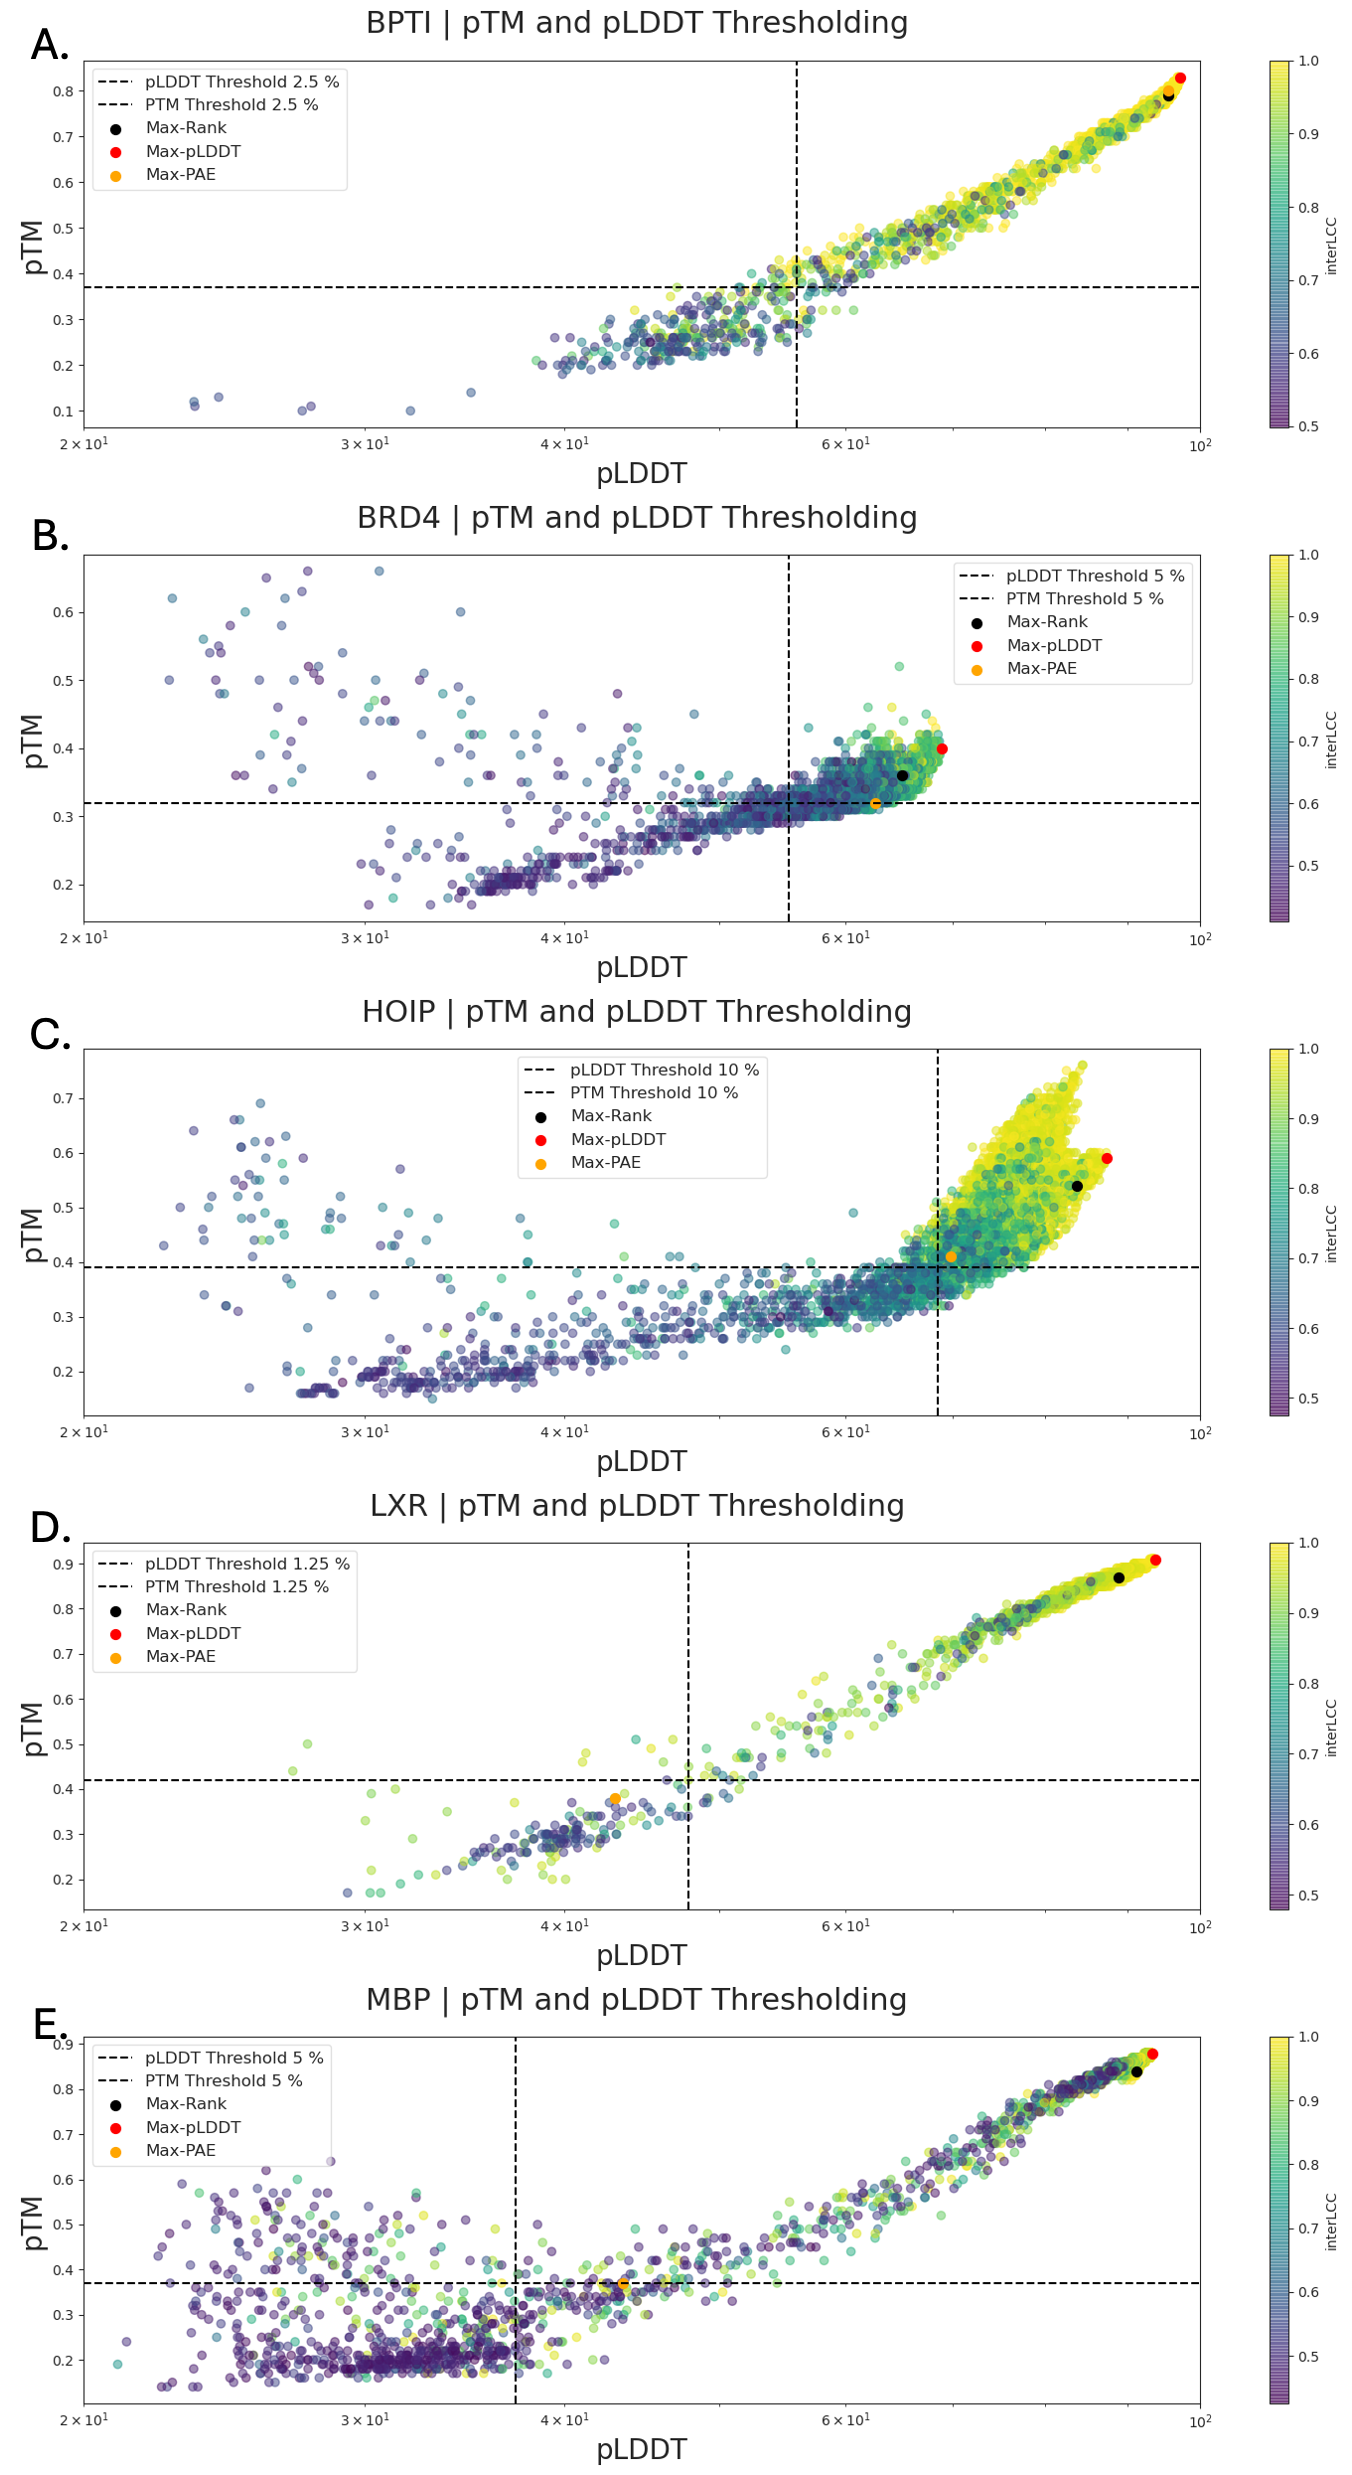
\includegraphics[width=0.58\textwidth, keepaspectratio]{valdx-af2-cleaning-confidence/fig.png}
    \caption[AF2-MSAss ensemble cleaning using confidence-based quality assessment]{AF2-MSAss ensemble cleaning using confidence-based quality assessment. Predicted Template Modelling (pTM) scores plotted against predicted Local Distance Difference Test (pLDDT) values for \textbf{(A)} BPTI, \textbf{(B)} BRD4, \textbf{(C)} HOIP, \textbf{(D)} LXR$\alpha$, and \textbf{(E)} MBP protein systems, with points coloured by structural local-distance Pearson correlation to the highest-pLDDT structure (Max-pLDDT). Confidence thresholds for structure filtering shown as dashed black lines, with threshold percentages set \textit{a priori}. Median values are shown by the dotted lines. Structures selected by the three criteria are labelled Max-Rank (black crosses), Max-pLDDT (red stars), and Max-PAE (orange triangles), denoting the highest-pLDDT structure in the 127-MSA subset, the highest-pLDDT structure in the complete ensemble, and the highest-PAE structure in the complete ensemble, respectively. PAE denotes predicted aligned error; higher values indicate lower confidence.}
    \label{fig:valdx-af2-confidence}
\end{figure}

\begin{figure}[htbp]
    \centering
    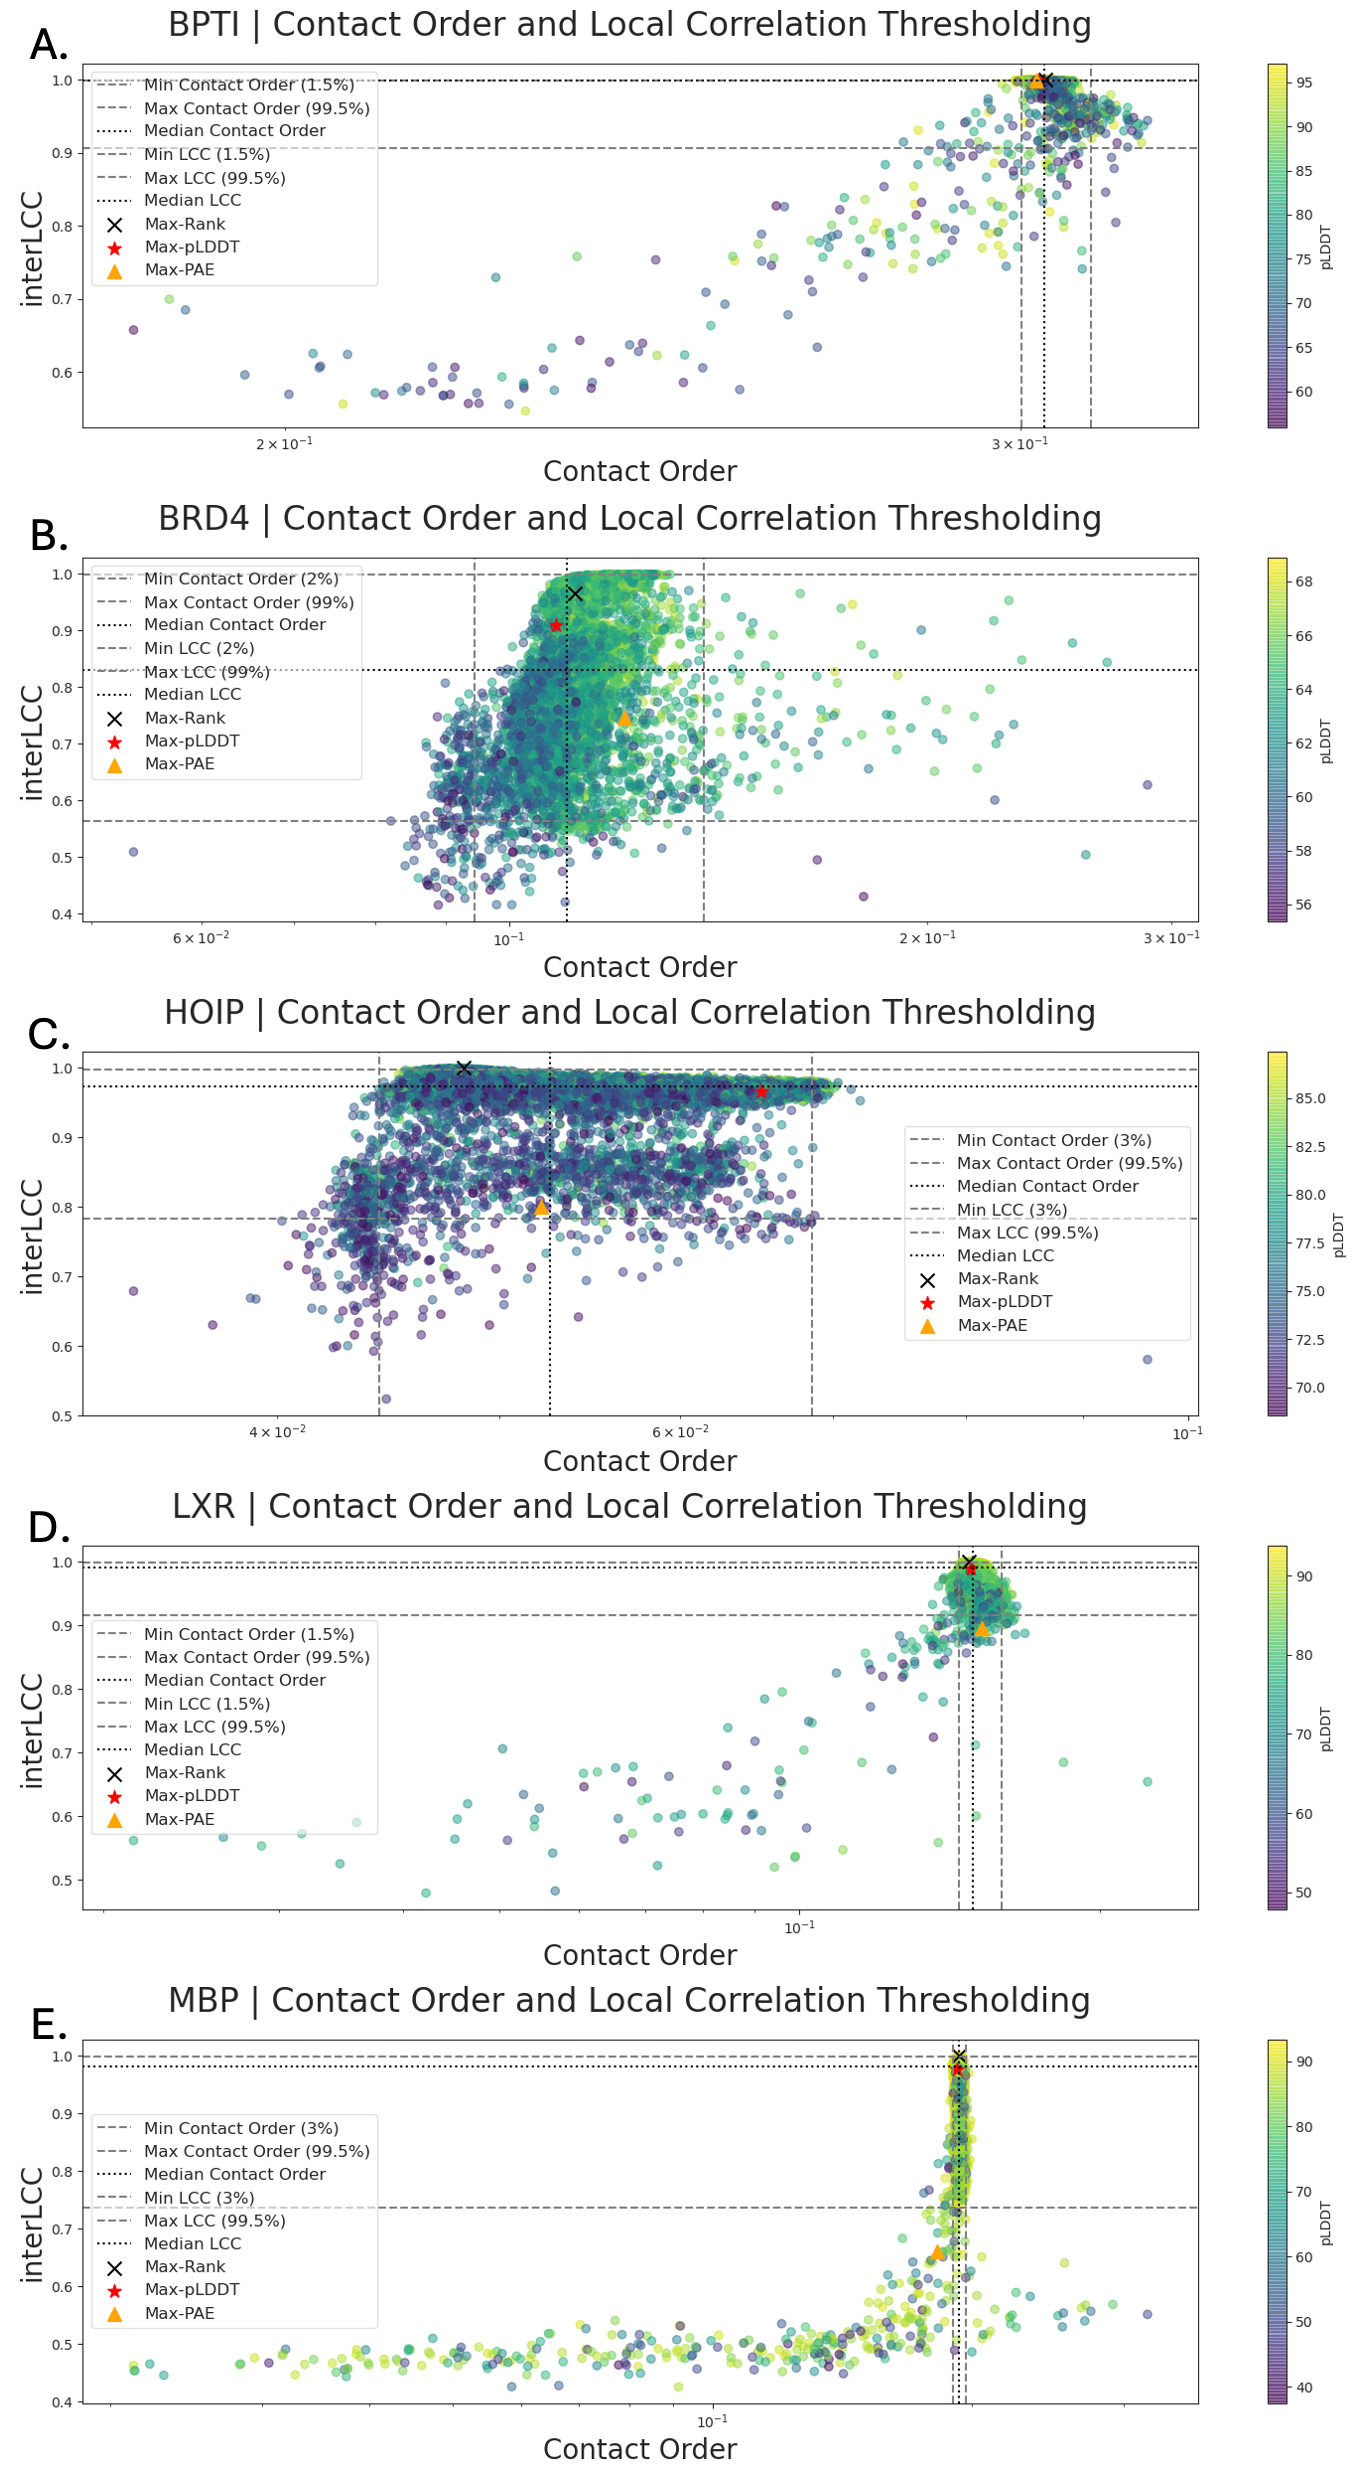
\includegraphics[width=0.60\textwidth, keepaspectratio]{valdx-af2-cleaning-contact-order/fig.png}
    \caption[AF2-MSAss ensemble cleaning using contact order and local correlation assessment]{AF2-MSAss ensemble cleaning using contact order and local correlation assessment across five protein systems. Contact Order plotted against reference-based structural local-distance correlation for \textbf{(A)} BPTI, \textbf{(B)} BRD4, \textbf{(C)} HOIP, \textbf{(D)} LXR$\alpha$, and \textbf{(E)} MBP protein systems, with points coloured by pLDDT confidence scores. Quality thresholds for structure filtering shown as grey dashed lines for minimum/maximum Contact Order and structural local-distance correlation, with percentile values varying by protein complexity. Median values indicated by black dotted lines. Structures selected by the three criteria are labelled Max-Rank (black crosses), Max-pLDDT (red stars), and Max-PAE (orange triangles), denoting the highest-pLDDT structure in the 127-MSA subset, the highest-pLDDT structure in the complete ensemble, and the highest-PAE structure in the complete ensemble, respectively. PAE denotes predicted aligned error; higher values indicate lower confidence. Results demonstrate systematic structural quality gradients, with well-folded proteins showing distinct high-confidence clusters while flexible proteins display broader distributions.}
    \label{fig:valdx-af2-contact-order}
\end{figure}

\paragraph{Structural local-distance correlation.}
We compared local geometry between structures using Pearson correlation of corresponding C$\alpha$--C$\alpha$ distance vectors. For structures $a$ and $b$, the comparison includes the same residue-pair indices in both vectors, restricted to pairs whose distances are at most $8\,\text{\AA}$ in both structures:
\begin{equation}
\begin{aligned}
d_{mn}^{(a)} &= \lVert\mathbf r_m^{(a)}-\mathbf r_n^{(a)}\rVert_2,\\
\mathcal N_{ab} &= \{(m,n):m<n,\ d_{mn}^{(a)}\leq8\,\text{\AA},\
d_{mn}^{(b)}\leq8\,\text{\AA}\}.
\end{aligned}
\label{eq:valdx-structural-ldc-pairs}
\end{equation}
\begin{equation}
L_{ab}=\operatorname{corr}_{\mathrm P}
\left([d_{mn}^{(a)}]_{(m,n)\in\mathcal N_{ab}},
[d_{mn}^{(b)}]_{(m,n)\in\mathcal N_{ab}}\right).
\label{eq:valdx-structural-ldc}
\end{equation}
Here, $\operatorname{corr}_{\mathrm P}$ denotes Pearson correlation, with corresponding residue pairs ordered identically in both vectors. The coefficient lies between $-1$ and $1$ when defined. It measures agreement between local distance patterns rather than correlated motion over frames.

For post-filter assessment, we calculate correlations between distinct structures selected nearest to the 20 K-means centroids in the first five principal components of the all-pair C$\alpha$ distance representation. The summary is the mean of the valid off-diagonal comparisons; self-comparisons are excluded. Representative selection requires mapping indices within the retained-frame array back to the original trajectory indices.

During filtering, each candidate structure is scored against a fixed reference using Pearson correlation of corresponding local C$\alpha$ distances. The cleaning figures identify this reference as the highest-pLDDT structure (Max-pLDDT); protein-specific correlation percentiles are listed in \cref{tab:valdx-af2-filter-thresholds}.

\subsection{Molecular Dynamics Setup and Equilibration}
\label{app:valdx-md-setup}

MD experiments were performed using GROMACS. Structures were protonated at pH 7 using GROMACS pdb2gmx with the AMBER ff14SB force field.\supercite{maierFf14SBImprovingAccuracy2015} The system was solvated using the TIP3P water model. Force-field parameters were chosen to match the original settings by the AMBER MD engine itself; simulation parameters and equilibration protocols were obtained from the repository supporting Kosarim et al.\supercite{kosarimMolecularDynamicsSimulations2024} Exact implementations used for this study can be found in the repositories in \cref{app:valdx-implementation}. Key simulation parameters are summarised in \cref{tab:valdx-md-parameters}.

\begin{table}[htbp]
    \centering
    \small
    \begin{tabular}{ll}
    \toprule
        \textbf{Parameter} & \textbf{Value} \\
        \midrule
        Force field & AMBER ff14SB \\
        Water model & TIP3P \\
        Protonation pH & 7.0 (pdb2gmx) \\
        Salt concentration & 0.15 M NaCl \\
        Thermostat & V-rescale \\
        Barostat & Parrinello-Rahman \\
        Temperature & 300 K \\
        Pressure & 1 bar \\
        Timestep & 2 fs \\
        Electrostatics & PME \\
        Cutoffs & 1.0 nm \\
        Constraints & H-bonds (LINCS) \\
        \bottomrule
    \end{tabular}
    \caption{MD simulation parameters.}
    \label{tab:valdx-md-parameters}
\end{table}

\paragraph{Minimisation and equilibration protocol.}
After topology generation, position restraints were modified to only cover $C_\alpha$ atoms from residues that are included by the experimental data. Position restraints on $C_\alpha$ atoms were applied during equilibration to prevent large backbone collapse when starting from diverse AF2 geometries, then gradually released over five stages (\cref{tab:valdx-md-equilibration}). Since the starting structures cover a wide range of shapes, topologies were generated for each structure separately.

\begin{table}[htbp]
    \centering
    \small
    \begin{tabular}{lcc}
    \toprule
        \textbf{Step} & \textbf{Length} & \textbf{Restraint force constant (kJ mol$^{-1}$ nm$^{-2}$)} \\
        \midrule
        Minimisation & $<$10000 steps & 500 \\
        EQ1 & 100 ps & 500 \\
        EQ2 & 200 ps & 500 \\
        EQ3 & 200 ps & 50 \\
        EQ4 & 200 ps & 5 \\
        EQ5 & 1 ns & 0 \\
        \bottomrule
    \end{tabular}
    \caption{Minimisation and equilibration schedule. Position restraints act on $C_\alpha$ atoms of residues covered by the experimental data.}
    \label{tab:valdx-md-equilibration}
\end{table}

\subsection{Single-Start, Multiple-Start and T-FES Protocols}
\label{app:valdx-md-protocols}

\paragraph{MD-1Start.}
We selected the single highest confidence AF2 structure and performed 5 replicates of 20 ns of production MD. This represents the standard approach of initiating simulation from a single, high-quality structure to test if conventional MD suffices to sample relevant states. To ensure the stability of the structures, 10 ns of unrestrained MD was additionally performed before the start of the production step.

\paragraph{MD-10Start.}
To represent a more diverse approach to generating ensembles with respect to HDX-MS data, the filtered AF2 (AF2-Filtered) ensemble was clustered by k-means ($k=10$), and the ten representative structures were used as diverse starting structures, which were then equilibrated using the same protocol as MD-1Start. To maintain a comparable computational budget to MD-1Start, each starting structure was run with a single replicate of 5 ns and 10 ns for relaxation and production simulations, respectively.

\paragraph{T-FES.}
To represent the most diverse range of fully plausible structures possible within a reasonable compute budget we modified an equilibrium-MD sampling approach, Frontier Expansion Sampling (FES).\supercite{zhangFrontierExpansionSampling2020} We adjusted the algorithm to concurrently sample across diverse starting structures with different topologies, producing multi-Topology Frontier Expansion Sampling (T-FES). To seed the initial conformations we combine both MD ensembles generated previously (MD-1Start and MD-10Start). We perform 20 cycles, capped at 200 short (0.1 ns) simulations per cycle which generates a maximum of 400 ns of short equilibrium-MD simulations. To maintain compatibility with the previous simulations the relevant GROMACS simulation files were converted into AMBER file formats compatible with OpenMM using ParmEd.\supercite{shirtsLessonsLearnedComparing2017} We retained OpenMM's default Langevin integrator, but added a Monte Carlo Barostat to match the Parrinello-Rahman barostat used in the GROMACS simulations. Each short simulation is preceded by an ultra-short equilibration (2000 steps, 1 fs time-step) to facilitate particle-velocity re-initialisation. The reported MD-TFES ensembles therefore use the modified multi-topology T-FES implementation with Monte Carlo barostat pressure coupling, distinct from the original Frontier-Expansion-Sampling codebase.

\section{Synthetic Data Generation and Simulator Validation}
\label{app:valdx-synthetic}
% TeaA state assignment and target construction.
% Kinetic simulator, numerical checks, digestion model,
% noise generation, clipping and seeds.

\section{Clustering and Structural Perturbation Algorithms}
\label{app:valdx-perturbations}
% PCA and clustering implementation.
% Exact noise, coordinate-mixing and proton-shuffling procedures.

\section{Experiment-Specific Fitting Protocols}
\label{app:valdx-case-studies}

Each list gives the inputs, optimised parameters, split replicates, $\gamma_\text{HDXer}$ grid and outputs of one experiment. Protocols are defined in \cref{tab:valdx-protocols}, split types in \cref{sec:valdx-splits} and metrics in \cref{sec:valdx-work}.

\begingroup
\raggedright

\subsection{Iso-Validation}
\label{app:valdx-case-iso}
\begin{itemize}
    \item \textbf{Inputs:} ISO-Bimodal and ISO-Trimodal ensembles; Synthetic HDX-uptake curves (generated from the ISO-Bimodal ensemble reweighted from 5\% to 40\% Open).
    \item \textbf{Optimised parameters:} Frame weights (RW-only).
    \item \textbf{Splits/Replicates:} 3 replicates $\times$ 4 split types (Non-Redundant, Spatial, Random, Sequential).
    \item \textbf{Optimisation grid:} $\gamma_\text{HDXer} \in \{1, \dots, 9\} \times 10^{\{-1, 0, 1\}}$.
    \item \textbf{Outputs computed:} $\text{MSE}_\text{Training}$, Apparent Work, Open State Recovery \%.
\end{itemize}

\subsection{Reweighting-Only}
\label{app:valdx-case-rw}
\begin{itemize}
    \item \textbf{Inputs:} Clustered ensembles (500 structures, k-means on PCA); HDX-MS Data (HDX-NMR for BPTI).
    \item \textbf{Optimised parameters:} Frame weights (RW-only).
    \item \textbf{Splits/Replicates:} 3 replicates $\times$ 2 split types (Non-Redundant, Spatial).
    \item \textbf{Optimisation grid:} $\gamma_\text{HDXer} \in \{1, \dots, 8\} \times 10^{0}$.
    \item \textbf{Outputs computed:} $W_1$ distance (AF2-Filtered vs.\ MD-1Start parent ensembles), $\text{MSE}_\text{Validation}$, $\Delta \text{MSE}_\text{opt}$, $\text{Work}_\text{shape}$, multivariate $\sigma$ (using $\text{Work}_\text{scale}$ and $\text{Work}_\text{density}$).
\end{itemize}

\subsection{BV-Model Parameter Optimisation}
\label{app:valdx-case-bv}
\begin{itemize}
    \item \textbf{Inputs:} Unclustered parent ensembles; HDX-MS Data.
    \item \textbf{Optimised parameters:} $\beta_C$, $\beta_H$ (BV-only).
    \item \textbf{Splits/Replicates:} 10 replicates $\times$ 2 split types (Non-Redundant, Spatial).
    \item \textbf{Outputs computed:} Optimal $\beta_C$, $\beta_H$ values, $\text{MSE}_\text{Validation}$.
\end{itemize}

\subsection{Protocol Comparison Benchmark}
\label{app:valdx-case-protocols}
\begin{itemize}
    \item \textbf{Inputs:} AF2-Filtered ensemble (500 structures); HDX-MS Data (HDX-NMR for BPTI).
    \item \textbf{Optimised parameters:} All protocols (BV-only, RW-only, RWafterBV, BVafterRW, MutualBVRW).
    \item \textbf{Splits/Replicates:} 3 replicates per stage.
    \item \textbf{Optimisation grid:} $\gamma_\text{HDXer} \in \{1, \dots, 8\} \times 10^{0}$ (for reweighting stages).
    \item \textbf{Outputs computed:} Comparative metrics across protocols.
\end{itemize}

\subsection{Kinetic Misspecification}
\label{app:valdx-case-kinetic}
\begin{itemize}
    \item \textbf{Inputs:} ISO-Bimodal ensemble clustered to 500 structures; synthetic peptide uptake generated at $\rho \in \{1000,1,0.01\}$.
    \item \textbf{Optimised parameters:} RW-only, RWafterBV, and BVafterRW, using the staged procedures of \cref{sec:valdx-fitting}.
    \item \textbf{Splits/Replicates:} 3 peptide-split replicates per kinetic condition; one matched noise realisation across conditions.
    \item \textbf{Optimisation grid:} $\gamma_\text{HDXer} \in \{1, \dots, 9\} \times 10^{0}$ (for reweighting stages).
    \item \textbf{Outputs computed:} Training and validation MSE, Open State Recovery, open-state populations, and Work Done metrics.
\end{itemize}

\subsection{Ensemble Size (Clustering) Sweep}
\label{app:valdx-case-clustering}
\begin{itemize}
    \item \textbf{Inputs:} Parent ensembles (10,000--12,700 structures), clustered to sizes \{0.1\%, 1\%, 5\%, 10\%, 20\%, 50\%, 100\%\}; HDX-MS Data (HDX-NMR for BPTI).
    \item \textbf{Optimised parameters:} Frame weights (RW-only).
    \item \textbf{Splits/Replicates:} 3 replicates $\times$ 2 split types.
    \item \textbf{Optimisation grid:} $\gamma_\text{HDXer} \in \{1, \dots, 8\} \times 10^{0}$.
    \item \textbf{Outputs computed:} Metrics vs Cluster Size.
\end{itemize}

\subsection{Structure Poisoning}
\label{app:valdx-case-poisoning}
\begin{itemize}
    \item \textbf{Inputs:} Clustered ensembles (1000 structures) + Poisoned structures (0.1\%, 1\%, 10\%, 50\%); HDX-MS Data.
    \item \textbf{Optimised parameters:} Frame weights (RW-only).
    \item \textbf{Splits/Replicates:} 3 replicates $\times$ 2 split types.
    \item \textbf{Optimisation grid:} $\gamma_\text{HDXer} \in \{1, \dots, 8\} \times 10^{0}$.
    \item \textbf{Outputs computed:} Correlation ($R$) and Standard Deviation ($SD$) of metrics.
\end{itemize}

\endgroup

\subsection{Curve-of-the-Knee Algorithm}
\label{app:valdx-knee}

\begin{algorithm}[htbp]
\caption{Curve-of-the-knee $\gamma_\text{HDXer}$ optimisation}
\label{alg:valdx-knee}
\footnotesize
\begin{algorithmic}[1]
\Require Set of candidate values $\gamma_\text{HDXer}= \{\gamma_1, \gamma_2, \ldots, \gamma_n\}$
\Require Corresponding error values $E = \{e_1, e_2, \ldots, e_n\}$
\Require Apparent work values $W = \{w_1, w_2, \ldots, w_n\}$
\Ensure Optimal $\gamma^*$
\State Initialize $x \leftarrow W$, $y \leftarrow E$
\State Sort data points by $x$ values
\If{$|x| = 1$}
    \State \Return $\gamma_1$
\ElsIf{$|x| = 0$}
    \State \textbf{raise} ValueError(``No valid gamma values found'')
\EndIf
\State $\gamma^* \leftarrow \text{null}$
\State \textit{// Method 1: Angle-based selection}
\State $\theta \leftarrow []$
\For{$i = 1$ to $|x|-1$}
    \State $\theta_i \leftarrow \arctan\left(\frac{y_{i+1} - y_i}{x_{i+1} - x_i}\right)$
    \State Append $\theta_i$ to $\theta$
\EndFor
\If{$\theta \neq []$}
    \State $\theta^* \leftarrow \arg\min_{\theta_i} |\theta_i + \pi/4|$
    \State $\gamma^* \leftarrow \gamma_{\text{index}(\theta^*)}$
\EndIf
\If{$\gamma^* = \text{null}$}
    \State \textit{// Method 2: Maximum distance from regression line}
    \State Fit linear regression: $\hat{y} = mx + b$ where $(m, b) = \text{polyfit}(x, y, 1)$
    \State $d \leftarrow []$
    \For{$i = 1$ to $|x|$}
        \State $d_i \leftarrow |y_i - (mx_i + b)|$
        \If{$y_i < mx_i + b$}
            \State $d_i \leftarrow -d_i$ \textit{// Negative for points below regression line}
        \EndIf
        \State Append $d_i$ to $d$
    \EndFor
    \State Filter: $d \leftarrow \{d_i : d_i < 0\}$ \textit{// Keep only negative distances}
    \If{$d \neq []$}
        \State $d^* \leftarrow \max\{|d_i| : d_i \in d\}$ \textit{// Maximum absolute negative distance}
        \State $\gamma^* \leftarrow \gamma_{\text{index}(d^*)}$
    \EndIf
\EndIf
\If{$\gamma^* = \text{null}$}
    \State \textit{// Method 3: Fallback to first valid gamma}
    \State $\gamma^* \leftarrow \min\{\gamma_i : e_i \text{ is finite}\}$
\EndIf
\State \Return $\gamma^*$
\end{algorithmic}
\end{algorithm}

\section{Supporting Mathematical and Statistical Details}
\label{app:valdx-mathematics}
% Regression specifications and complete statistical tables.

\subsection{Work Done Metrics}
\label{app:valdx-work-definitions}

The Work Done metrics of \cref{sec:valdx-work} are reported in energy units but do not represent thermodynamic work or changes in protein enthalpy or entropy. Changes in either direction contribute positively. Their energy scale comes from the EX2 regime. With the predominantly closed-state approximation, the opening free energy of residue $i$ is approximately $RT\ln P_{f,i}$ (\cref{eq:bg-opening-free-energy}). The EX2 relation motivates expressing log-protection changes on an $RT$ energy scale. The Work Done metrics are nevertheless defined as statistical comparisons of protection profiles. Each profile is the ensemble-averaged BV log protection factor of \cref{eq:bg-bv-average}, calculated with that ensemble-model's own frame weights and BV coefficients.

Mean-centring separates changes in relative protection from shifts in overall protection. Each residue's absolute deviation from the mean log protection factor, scaled by $RT$, gives its centred protection score. The same deviations define a residue weight and an entropy-like contribution. Centring and weights are calculated separately for each profile over the same matched residues. Because $w_\text{opt}(X;i)=e^{-a_i}\sum_{j=1}^{N}e^{-a_j}$, the weights sum to $\left(\sum_{i=1}^{N}e^{-a_i}\right)^2$ rather than to one, and $S_\text{opt}(X;i)$ is negative wherever $w_\text{opt}(X;i)>1$.

Work opt combines the centred score and the entropy-like contribution within each residue before taking the absolute value. By the triangle inequality, $\text{Work}_\text{opt}\le\text{Work}_\text{shape}+\text{Work}_\text{density}$. The same expressions compare any two profiles $X_1$ and $X_2$ over matched residues by substituting them for $X$ and $\hat X$.

\subsection{Structural Comparison Metrics}
\label{app:valdx-structural-metrics}

\paragraph{Local mean pair-distance RMS difference.}
For each residue $i$, we construct a neighbourhood $\mathcal S_i$ from ensemble 1's mean coordinates. Within that fixed neighbourhood, we calculate the mean distance of each unique C$\alpha$ residue pair separately in each ensemble and then take the RMS difference between those means,
\begin{equation}
    \overline d_{ab}^{\,X}=\frac{1}{|X|}
    \sum_{x\in X}\lVert\mathbf r_a(x)-\mathbf r_b(x)\rVert_2,
    \label{eq:valdx-mean-pair-distance}
\end{equation}
\begin{equation}
    D_i(X_1,X_2)=
    \sqrt{\frac{1}{M_i}
    \sum_{\substack{a<b\\a,b\in\mathcal S_i}}
    \left(\overline d_{ab}^{\,X_1}-\overline d_{ab}^{\,X_2}\right)^2},
    \qquad M_i=\binom{|\mathcal S_i|}{2}.
    \label{eq:valdx-pair-rms}
\end{equation}
This unweighted quantity measures differences in local ensemble-mean pair distances, in \text{\AA}. Pair distances are invariant to rigid translation and rotation of individual structures; neighbourhood selection from mean Cartesian coordinates nevertheless depends on how those coordinates were prepared. Because the neighbourhood is selected from ensemble 1, reversing the ensemble order can change the neighbourhood and the resulting value.

\paragraph{Residue-averaged Wasserstein-1 distance.}
For residue $i$, the C$\alpha$ distances to every C$\alpha$ atom, including its zero distance to itself, are pooled over all frames of ensemble $X$,
\begin{equation}
    \Omega_i(X)=\left\{\lVert\mathbf r_i(x)-\mathbf r_j(x)\rVert_2 : j=1,\dots,N,\ x\in X\right\}.
    \label{eq:valdx-w1-pool}
\end{equation}
Frames are unweighted. As $W_1$ is computed between normalised distributions, each pool is smoothed by a Gaussian kernel density estimate (KDE), $\hat f_i^{X}$. SciPy's KDE implementation uses Scott's rule for bandwidth selection.\supercite{virtanenSciPy10Fundamental2020} Both densities are evaluated on a common grid of $K=1000$ evenly spaced points $g_1<\dots<g_K$ spanning the pooled distances of both ensembles and normalised over that grid, giving $p_{i,k}^{X}=\hat f_i^{X}(g_k)/\sum_{l=1}^{K}\hat f_i^{X}(g_l)$ and cumulative distributions $F_{i,k}^{X}=\sum_{l\le k}p_{i,l}^{X}$. The residue distance and its average over the $N$ compared residues are
\begin{equation}
    W_{1,i}(X_1,X_2)=\sum_{k=1}^{K-1}\left|F_{i,k}^{X_1}-F_{i,k}^{X_2}\right|\left(g_{k+1}-g_k\right),
    \qquad
    \langle W_1(X_1,X_2)\rangle=\frac{1}{N}\sum_{i=1}^{N}W_{1,i}(X_1,X_2),
    \label{eq:valdx-w1}
\end{equation}
in \text{\AA}. Values approaching zero indicate identical pooled distance distributions, and larger values indicate divergence between them.

\paragraph{Weighted RMSF.}
To account for the non-uniform weights of structures in the ensemble, the weighted RMSF for residue $i$ is computed as
\begin{equation}
    \text{RMSF}_i(X)=\sqrt{\sum_{x\in X}p(x)\left\lVert\mathbf r_i(x)-\langle\mathbf r_i(X)\rangle\right\rVert^2},
    \qquad
    \langle\mathbf r_i(X)\rangle=\sum_{x\in X}p(x)\,\mathbf r_i(x),
    \label{eq:valdx-weighted-rmsf}
\end{equation}
where $p(x)$ is the weight of structure $x$ in ensemble $X$.

\paragraph{Dynamical local cross-correlation.}
For each ensemble $X$, we define the displacement of residue $i$ relative to its mean C$\alpha$ position and calculate its normalised displacement covariance with residue $j$,
\begin{equation}
\begin{aligned}
    \delta\mathbf r_i(t)&=\mathbf r_i(t)-\langle\mathbf r_i\rangle_t,\\
    C_{ij}(X)&=
    \frac{\langle\delta\mathbf r_i(t)\cdot\delta\mathbf r_j(t)\rangle_t}
    {\sqrt{\langle\lVert\delta\mathbf r_i(t)\rVert_2^2\rangle_t
    \langle\lVert\delta\mathbf r_j(t)\rVert_2^2\rangle_t}}.
\end{aligned}
    \label{eq:valdx-dynamical-pair-correlation}
\end{equation}
Averages are unweighted averages over ensemble frames. Trajectories were aligned on C$\alpha$ atoms before analysis. Spatial neighbours are identified using the mean inter-residue distance over frames,
\begin{equation}
    \mathcal N_i(X)=\left\{j\ne i:
    \left\langle\lVert\mathbf r_i(t)-\mathbf r_j(t)\rVert_2\right\rangle_t
    \leq8\,\text{\AA}\right\}.
    \label{eq:valdx-lcc-neighbours}
\end{equation}
The residue-level LCC is the arithmetic mean of the defined pair correlations within this neighbourhood,
\begin{equation}
    \mathrm{LCC}_i(X)=\frac{1}{|\mathcal V_i(X)|}
    \sum_{j\in\mathcal V_i(X)}C_{ij}(X),
    \qquad
    \mathcal V_i(X)=\{j\in\mathcal N_i(X):C_{ij}(X)\text{ is defined}\}.
    \label{eq:valdx-lcc}
\end{equation}
Undefined pair correlations, including those arising from zero displacement variance, are excluded. A residue with no valid pair correlations has no defined neighbourhood mean. Neighbourhood means are shown in \cref{app:valdx-supporting-results} with bands spanning one standard deviation across the contributing pair correlations. These bands describe variation among neighbours, rather than sampling uncertainty in the mean.

\section{Extended Ensemble Characterisation and Sensitivity Analyses}
\label{app:valdx-supporting-results}
% Additional structural comparisons, replicate plots,
% per-protein results and sensitivity analyses.

\section{Computational Implementation and Data Availability}
\label{app:valdx-implementation}
% Software versions, commits, hardware, code and data locations.
